\documentclass[border=10pt]{standalone}

\usepackage{tikz}
\usepackage{tikzsymbols}
\usetikzlibrary{calc,patterns,shapes.geometric}

\def\centerarc[#1](#2)(#3:#4:#5){\draw[#1] ($(#2)+({#5*cos(#3)},{#5*sin(#3)})$) arc (#3:#4:#5);}

\begin{document}
	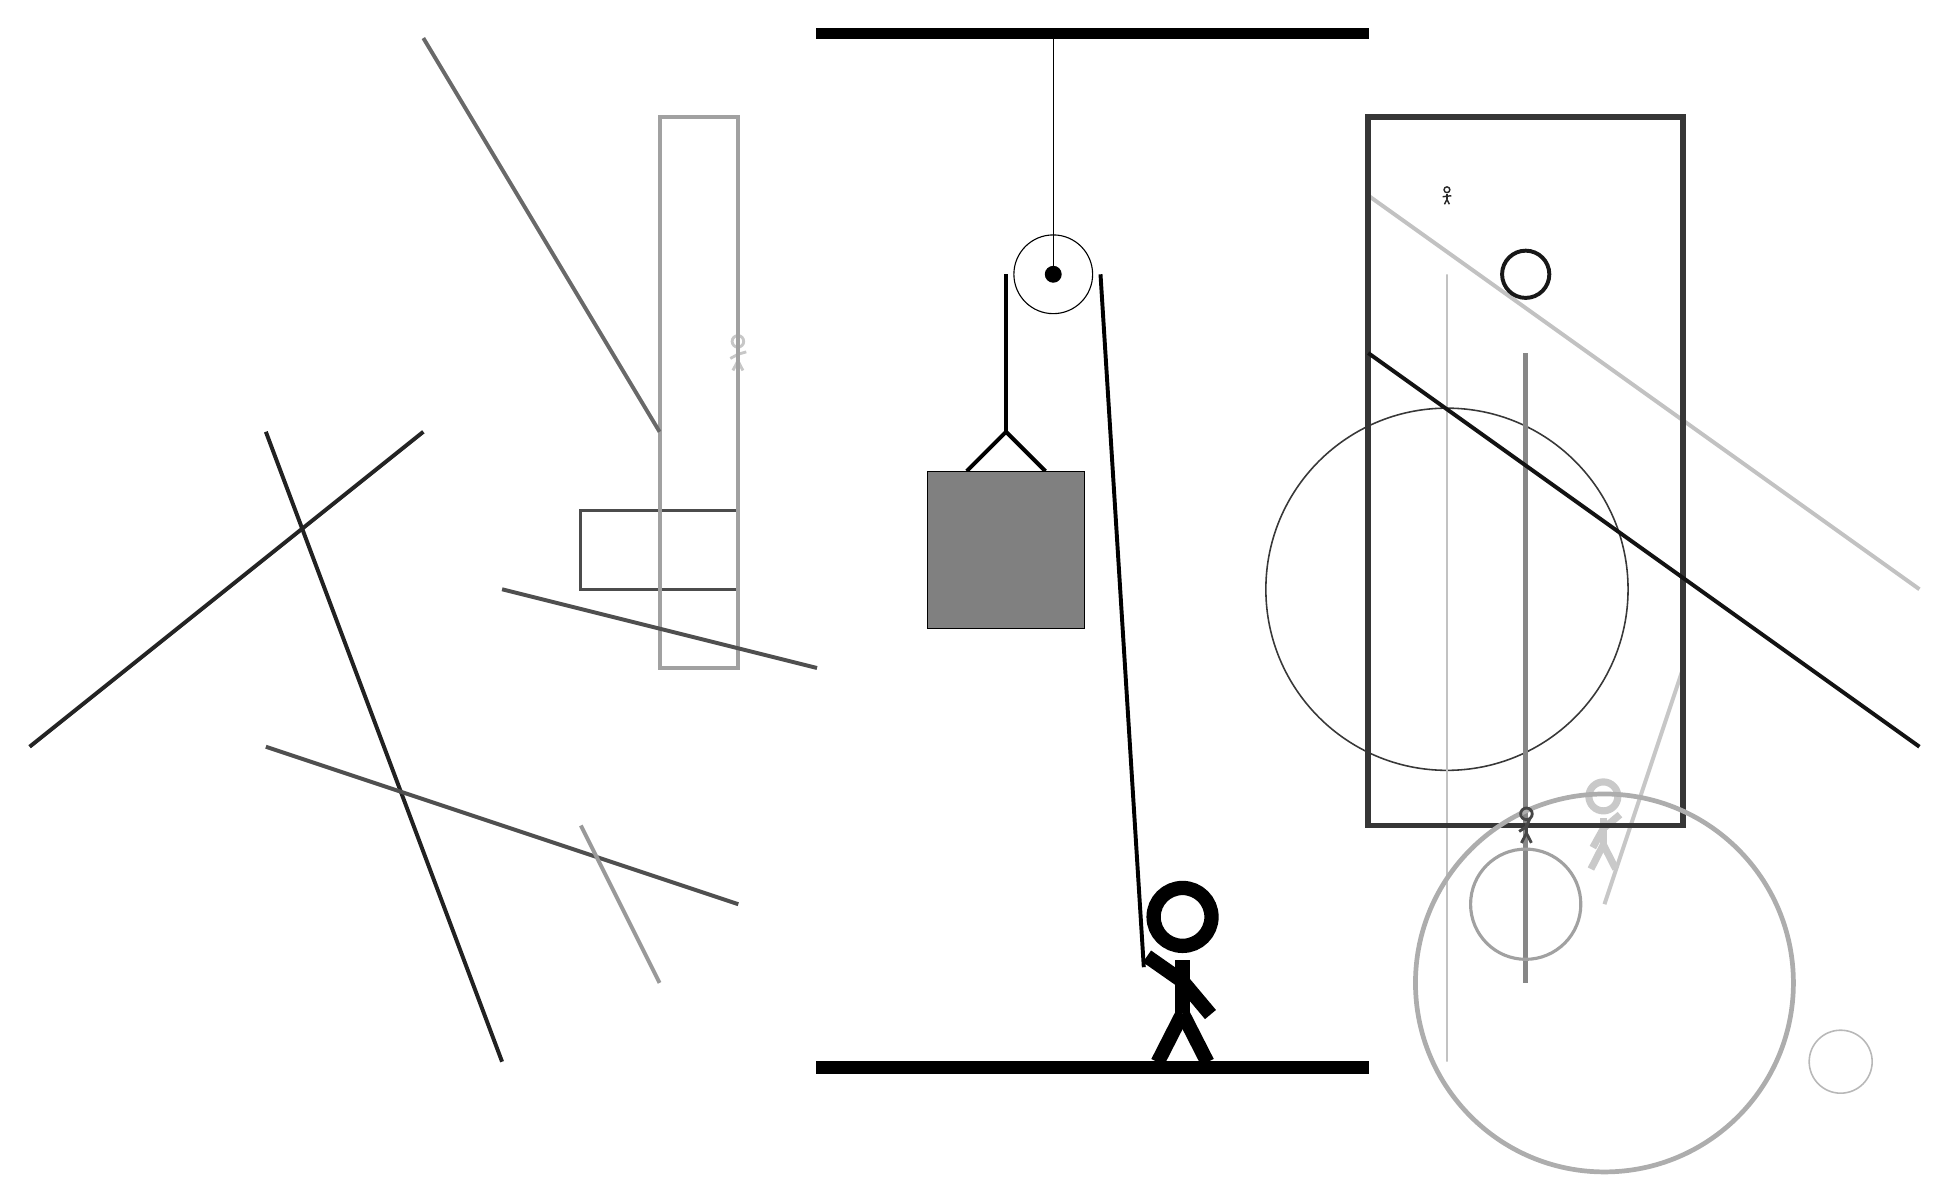
\begin{tikzpicture}
		%%%%% START %%%%%
		
		\draw[fill=black] (-2, 10) rectangle (5, 10.125);
		
		\draw (1, 7) circle (0.5);
		\draw[fill=black] (1, 7) circle (0.1);
		\draw (1, 10) -- (1, 7);
		
		\draw[line width=0.5mm] (-0.1, 4.5) -- (0.4, 5.0) -- (0.9, 4.5);
		\draw[fill=black!50] (-0.6, 4.5) rectangle (1.4, 2.5);
		
		\draw[line width=0.5mm] (0.4, 7) -- (0.4, 5.0);
		\centerarc[line width=0.5mm](1, 7)(0:180:0.6);
		\draw[line width=0.5mm](1.6, 7) -- (2.15, -1.8);
		
		\node at (2.6, -1.9) {\Strichmaxerl[10][-35][-50]};
		
		\draw[line width=0.5mm, color=black!87](-6, -3) -- (-9, 5);
		
		\draw[line width=0.5mm, color=black!24](5, 8) -- (12, 3);
		\draw [line width=0.2mm, color=black!78](6, 3) circle (2.3);
		\draw[line width=0.5mm, color=black!22](8, -1) -- (9, 2);
		\draw[line width=0.4mm, color=black!70] (-3, 3) rectangle (-5, 4);
		\node[line width=0.6mm, color=black!21] at (8, 0) {\Strichmaxerl[5][61][40]};
		
		\draw[line width=0.5mm, color=black!69](-3, -1) -- (-9, 1);
		
		\draw[line width=0.7mm, color=black!35] (7, -2) rectangle (7, 2);
		\draw[line width=0.6mm, color=black!47] (7, 6) rectangle (7, -2);
		
		\node[line width=0.7mm, color=black!22] at (-3, 6) {\Strichmaxerl[2][29][16]};
		
		\draw[line width=0.5mm, color=black!86](-7, 5) -- (-12, 1);
		\node[line width=0.4mm, color=black!85] at (6, 8) {\Strichmaxerl[1][8][5]};
		\draw[line width=0.5mm, color=black!90](-4, 9) -- (-4, 7);
		\draw[line width=0.2mm, color=black!24] (6, -3) rectangle (6, 7);
		\draw [line width=0.2mm, color=black!28](11, -3) circle (0.4);
		\draw [line width=0.4mm, color=black!37](7, -1) circle (0.7);
		
		\draw[line width=0.7mm, color=black!79] (5, 0) rectangle (9, 9);
		\draw [line width=0.6mm, color=black!32](8, -2) circle (2.4);
		\draw[line width=0.5mm, color=black!40](-5, 0) -- (-4, -2);
		\draw[line width=0.5mm, color=black!37] (-4, 2) rectangle (-3, 9);
		\draw[line width=0.5mm, color=black!69](-6, 3) -- (-2, 2);
		
		\draw[line width=0.5mm, color=black!59](-7, 10) -- (-4, 5);
		
		\draw [line width=0.5mm, color=black!91](7, 7) circle (0.3);
		\node[line width=0.4mm, color=black!72] at (7, 0) {\Strichmaxerl[2][33][67]};
		\draw[line width=0.5mm, color=black!93](5, 6) -- (12, 1);
		
		
		\draw[fill=black] (-2, -3) rectangle (5, -3.15);
		
		%%%%% END %%%%%
	\end{tikzpicture}
\end{document}